
%(BEGIN_QUESTION)
% Copyright 2011, Tony R. Kuphaldt, released under the Creative Commons Attribution License (v 1.0)
% This means you may do almost anything with this work of mine, so long as you give me proper credit

Anta at du skal sjekke integriteten i en flerleder signalkabel mellom to steder. Kabelen har seks signalledere pluss skjerm, terminert i klemrekker i begge ender:

$$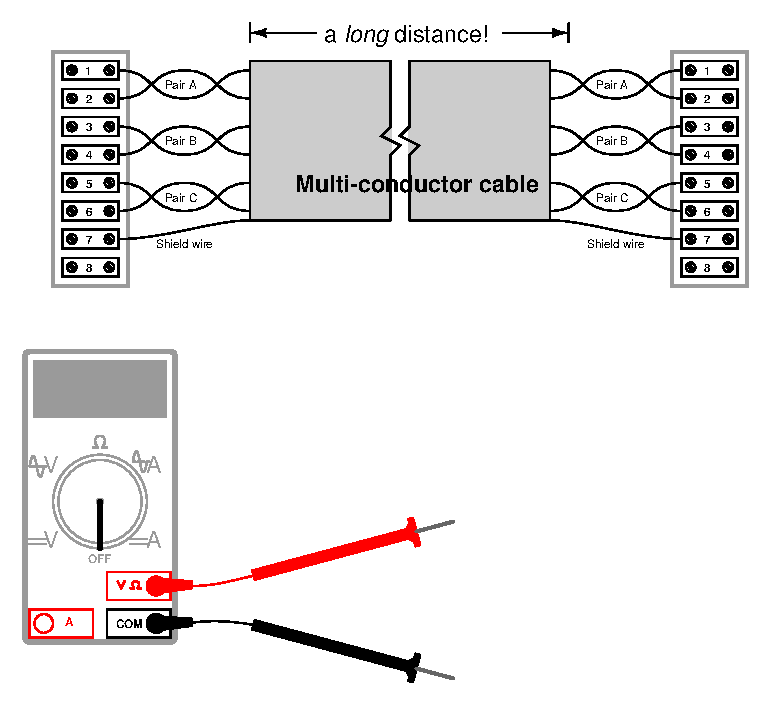
\includegraphics[width=15.5cm]{i00734x01.eps}$$

Feil du leter etter er {\it brudd} i ledere, samt {\it kortslutninger} mellom ledere og/eller til jord. Beskriv en testsekvens du kan gjøre kun med multimeter for å kontrollere kabelens elektriske integritet.

\vfil

\underbar{file i00734}
\eject
%(END_QUESTION)





%(BEGIN_ANSWER)

Dette er en vurdert oppgave -- ingen svar eller hint er gitt!

%(END_ANSWER)





%(BEGIN_NOTES)

Siden kabelen er lang, rekker ikke måleledningene mellom endene. Derfor må testen settes opp slik at måling kan gjøres fra én ende.

En metode er å sammenkoble alle seks lederne i den fjerne enden og deretter måle kontinuitet mellom lederpar i nær enden for å finne brudd. Hvis forventet kontinuitet mangler, er det brudd.

For kortslutningstester må lederne være separert. Mål deretter kontinuitet mellom alle lederpar og mot jord/skjerm. Kontinuitet der det ikke skal være det betyr kortslutning.

%INDEX% Elektronikkrepetisjon: kontinuitetstest av flerlederkabel

%(END_NOTES)
